% !TEX root = ../thesis.tex
\chapter{Implementation of a Relevant Algorithm}
\label{app:implementation_algorithm}

% Code listings should live in a code file, not embedded directly into your LaTeX code!
\lstinputlisting[language=c, caption={An implementation of an important algorithm from our work.}]{./listings/hello_world.c}


\chapter{Supplementary Data}
\label{app:supplementary_data}

The results of large ablative studies can often take up a lot of space, even with neat visualisation and formatting.
Consider putting full results in an appendix chapter and showing excerpts of interesting results in your chapters with detailed analysis.
You can use labels and references to refer the reader here for the full data.

\chapter{Web App Pages}
\label{app:web_designs}

\begin{figure}[h]
	\centering
	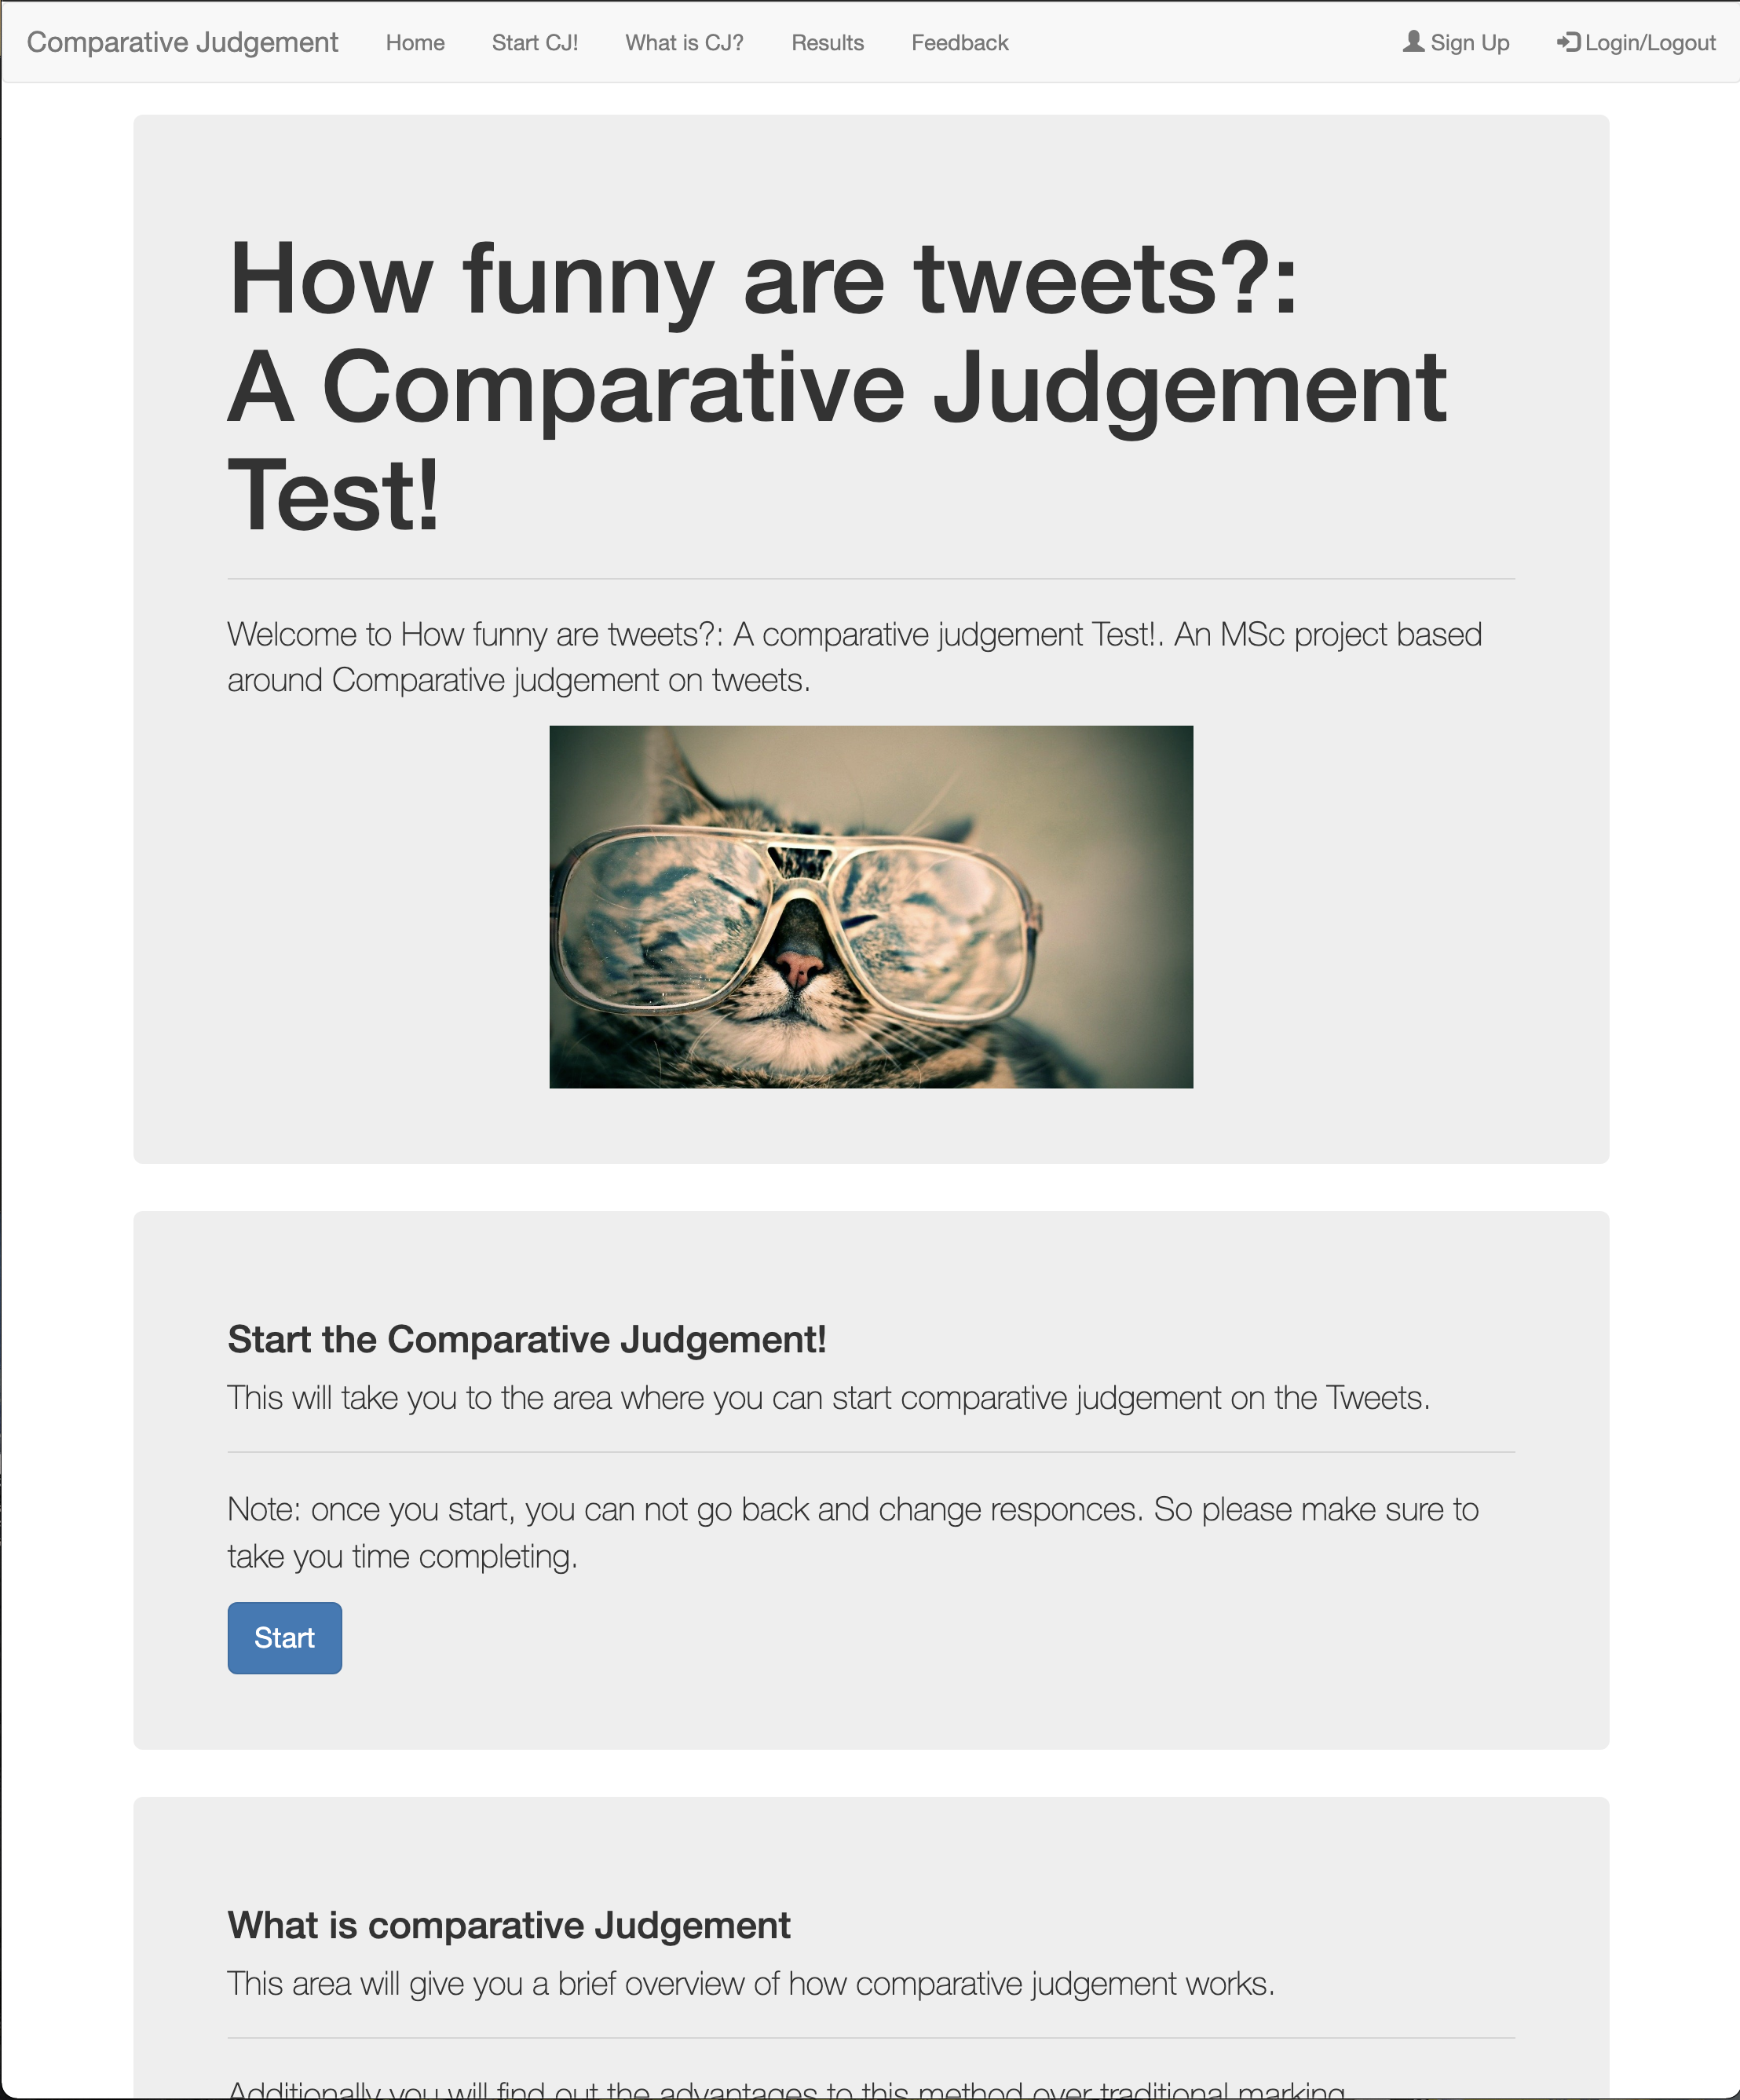
\includegraphics[width=10cm]{Home_page.png}
	\caption{}
	
		
	\end{figure} 
\begin{figure}[h]
	\centering
	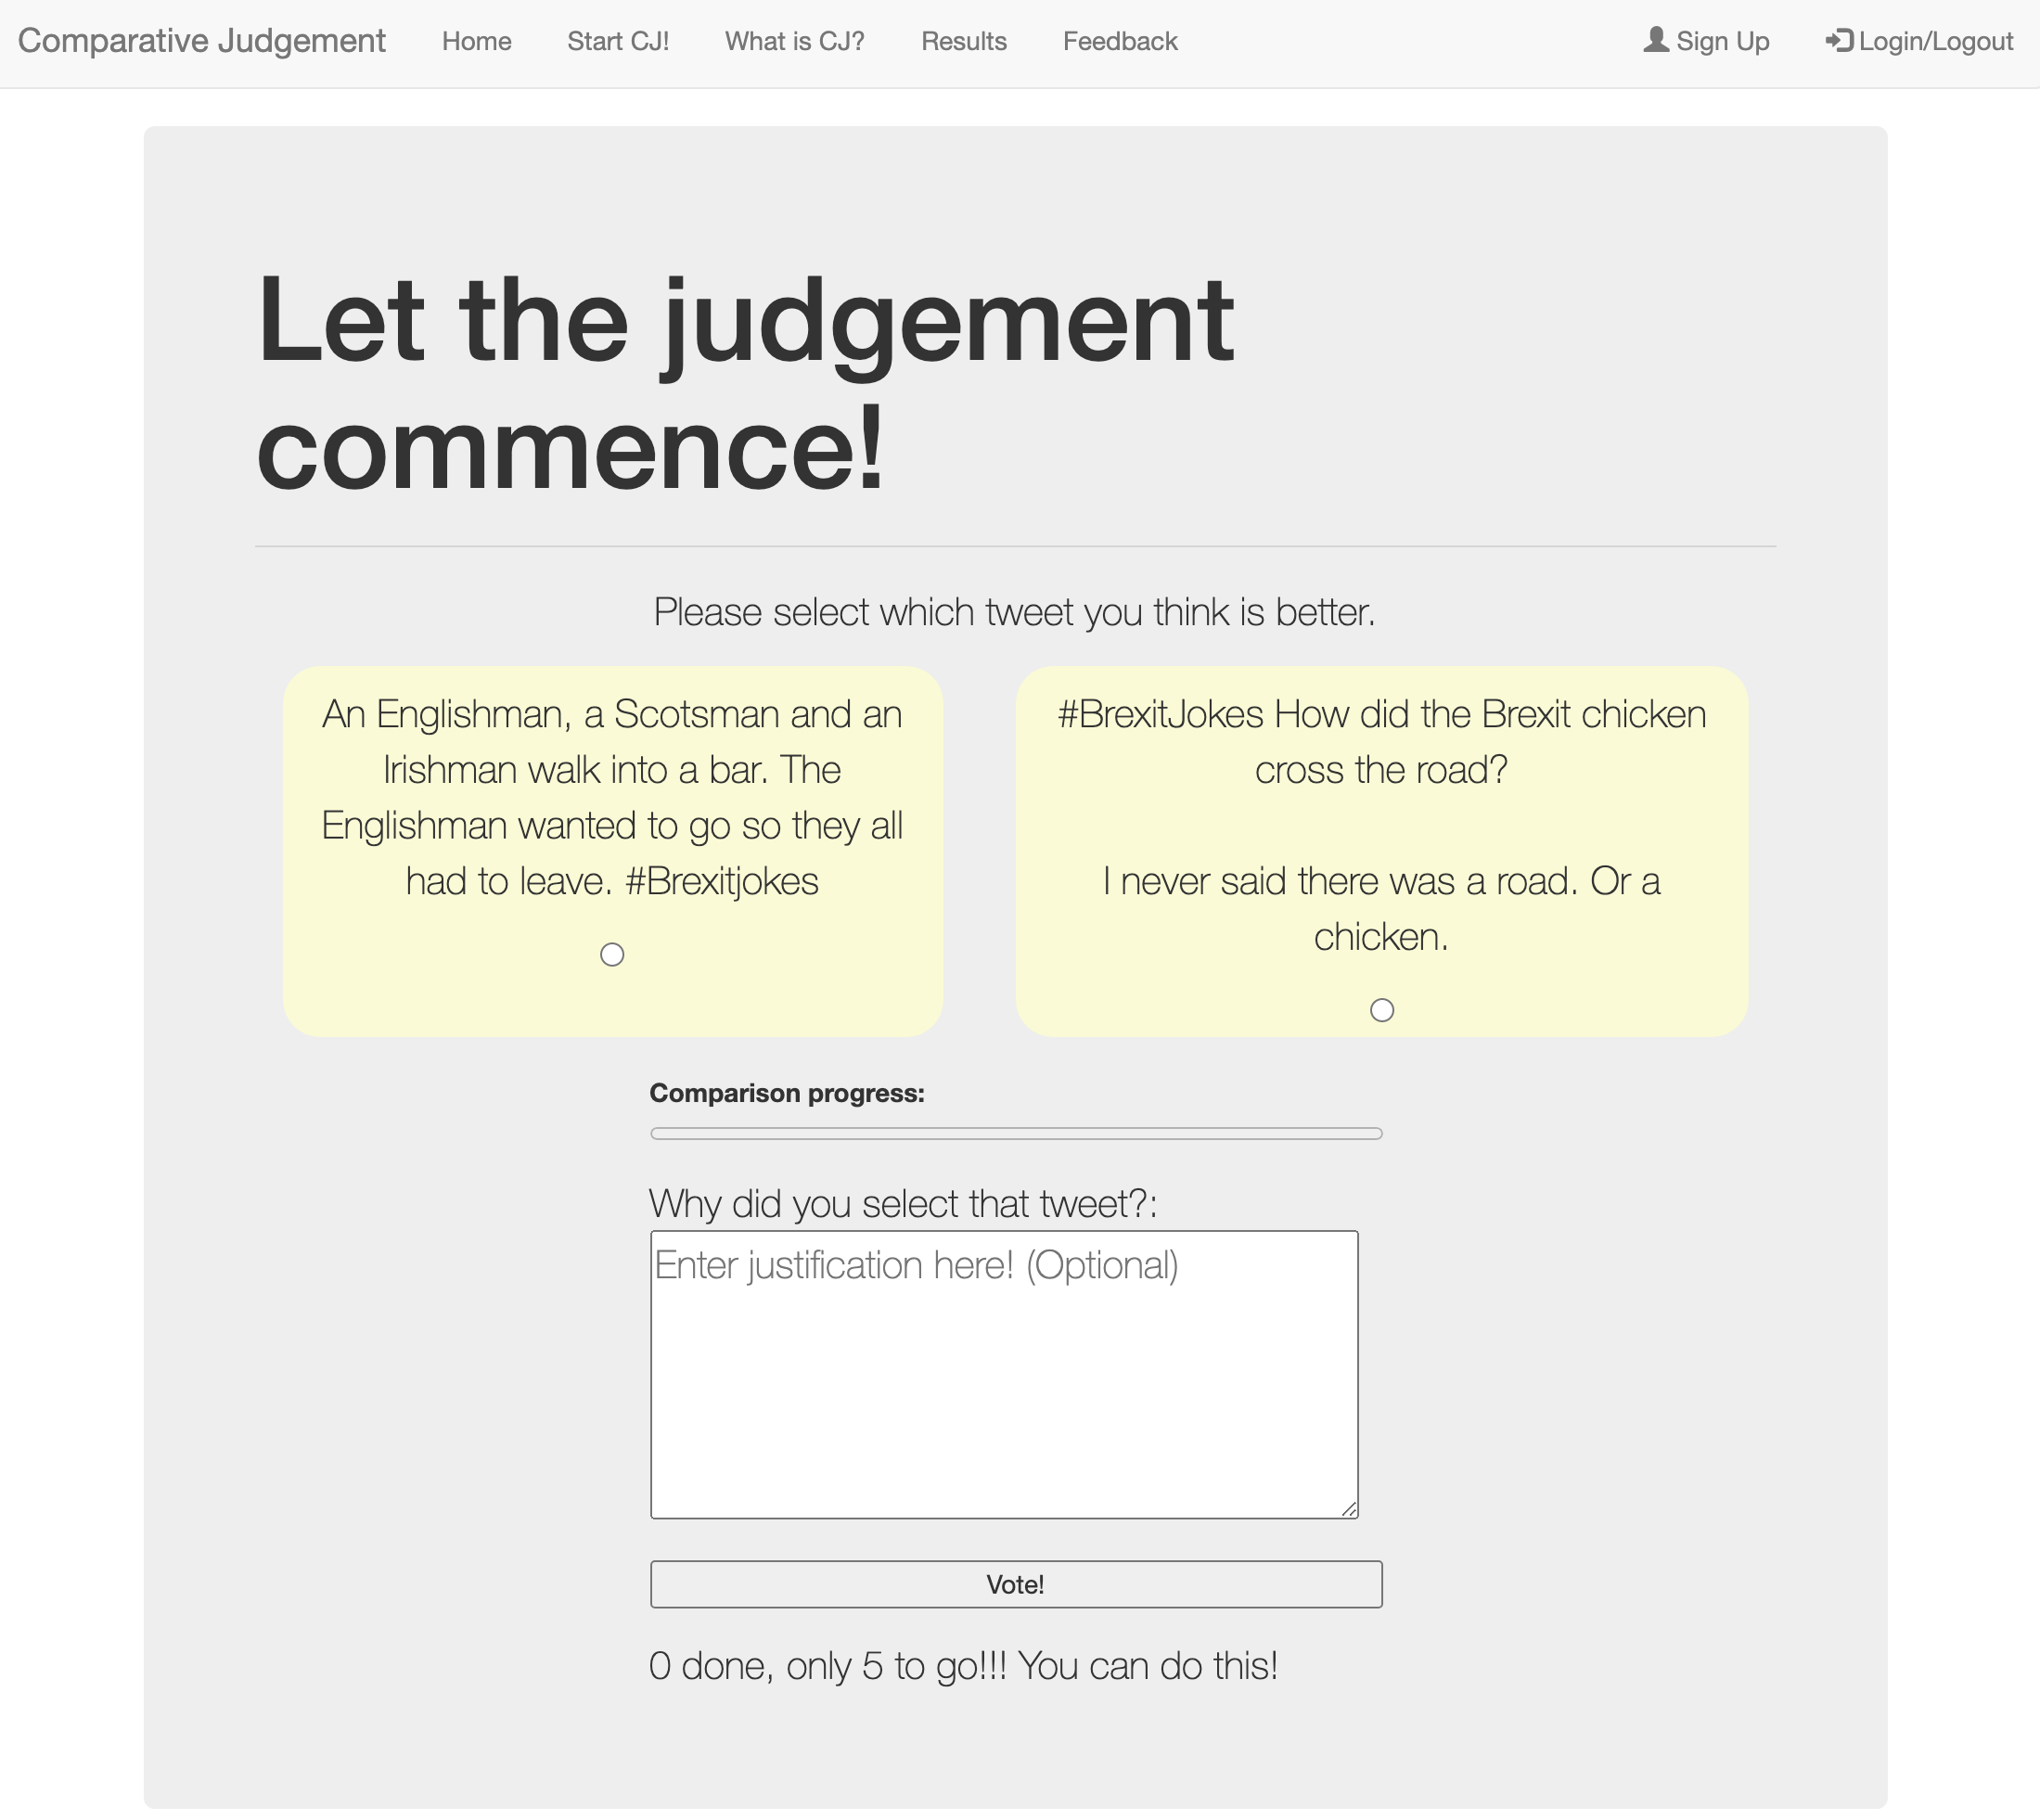
\includegraphics[width=10cm]{Compare.png}
	\caption{}
	
		
	\end{figure} 

\begin{figure}[h]
	\centering
	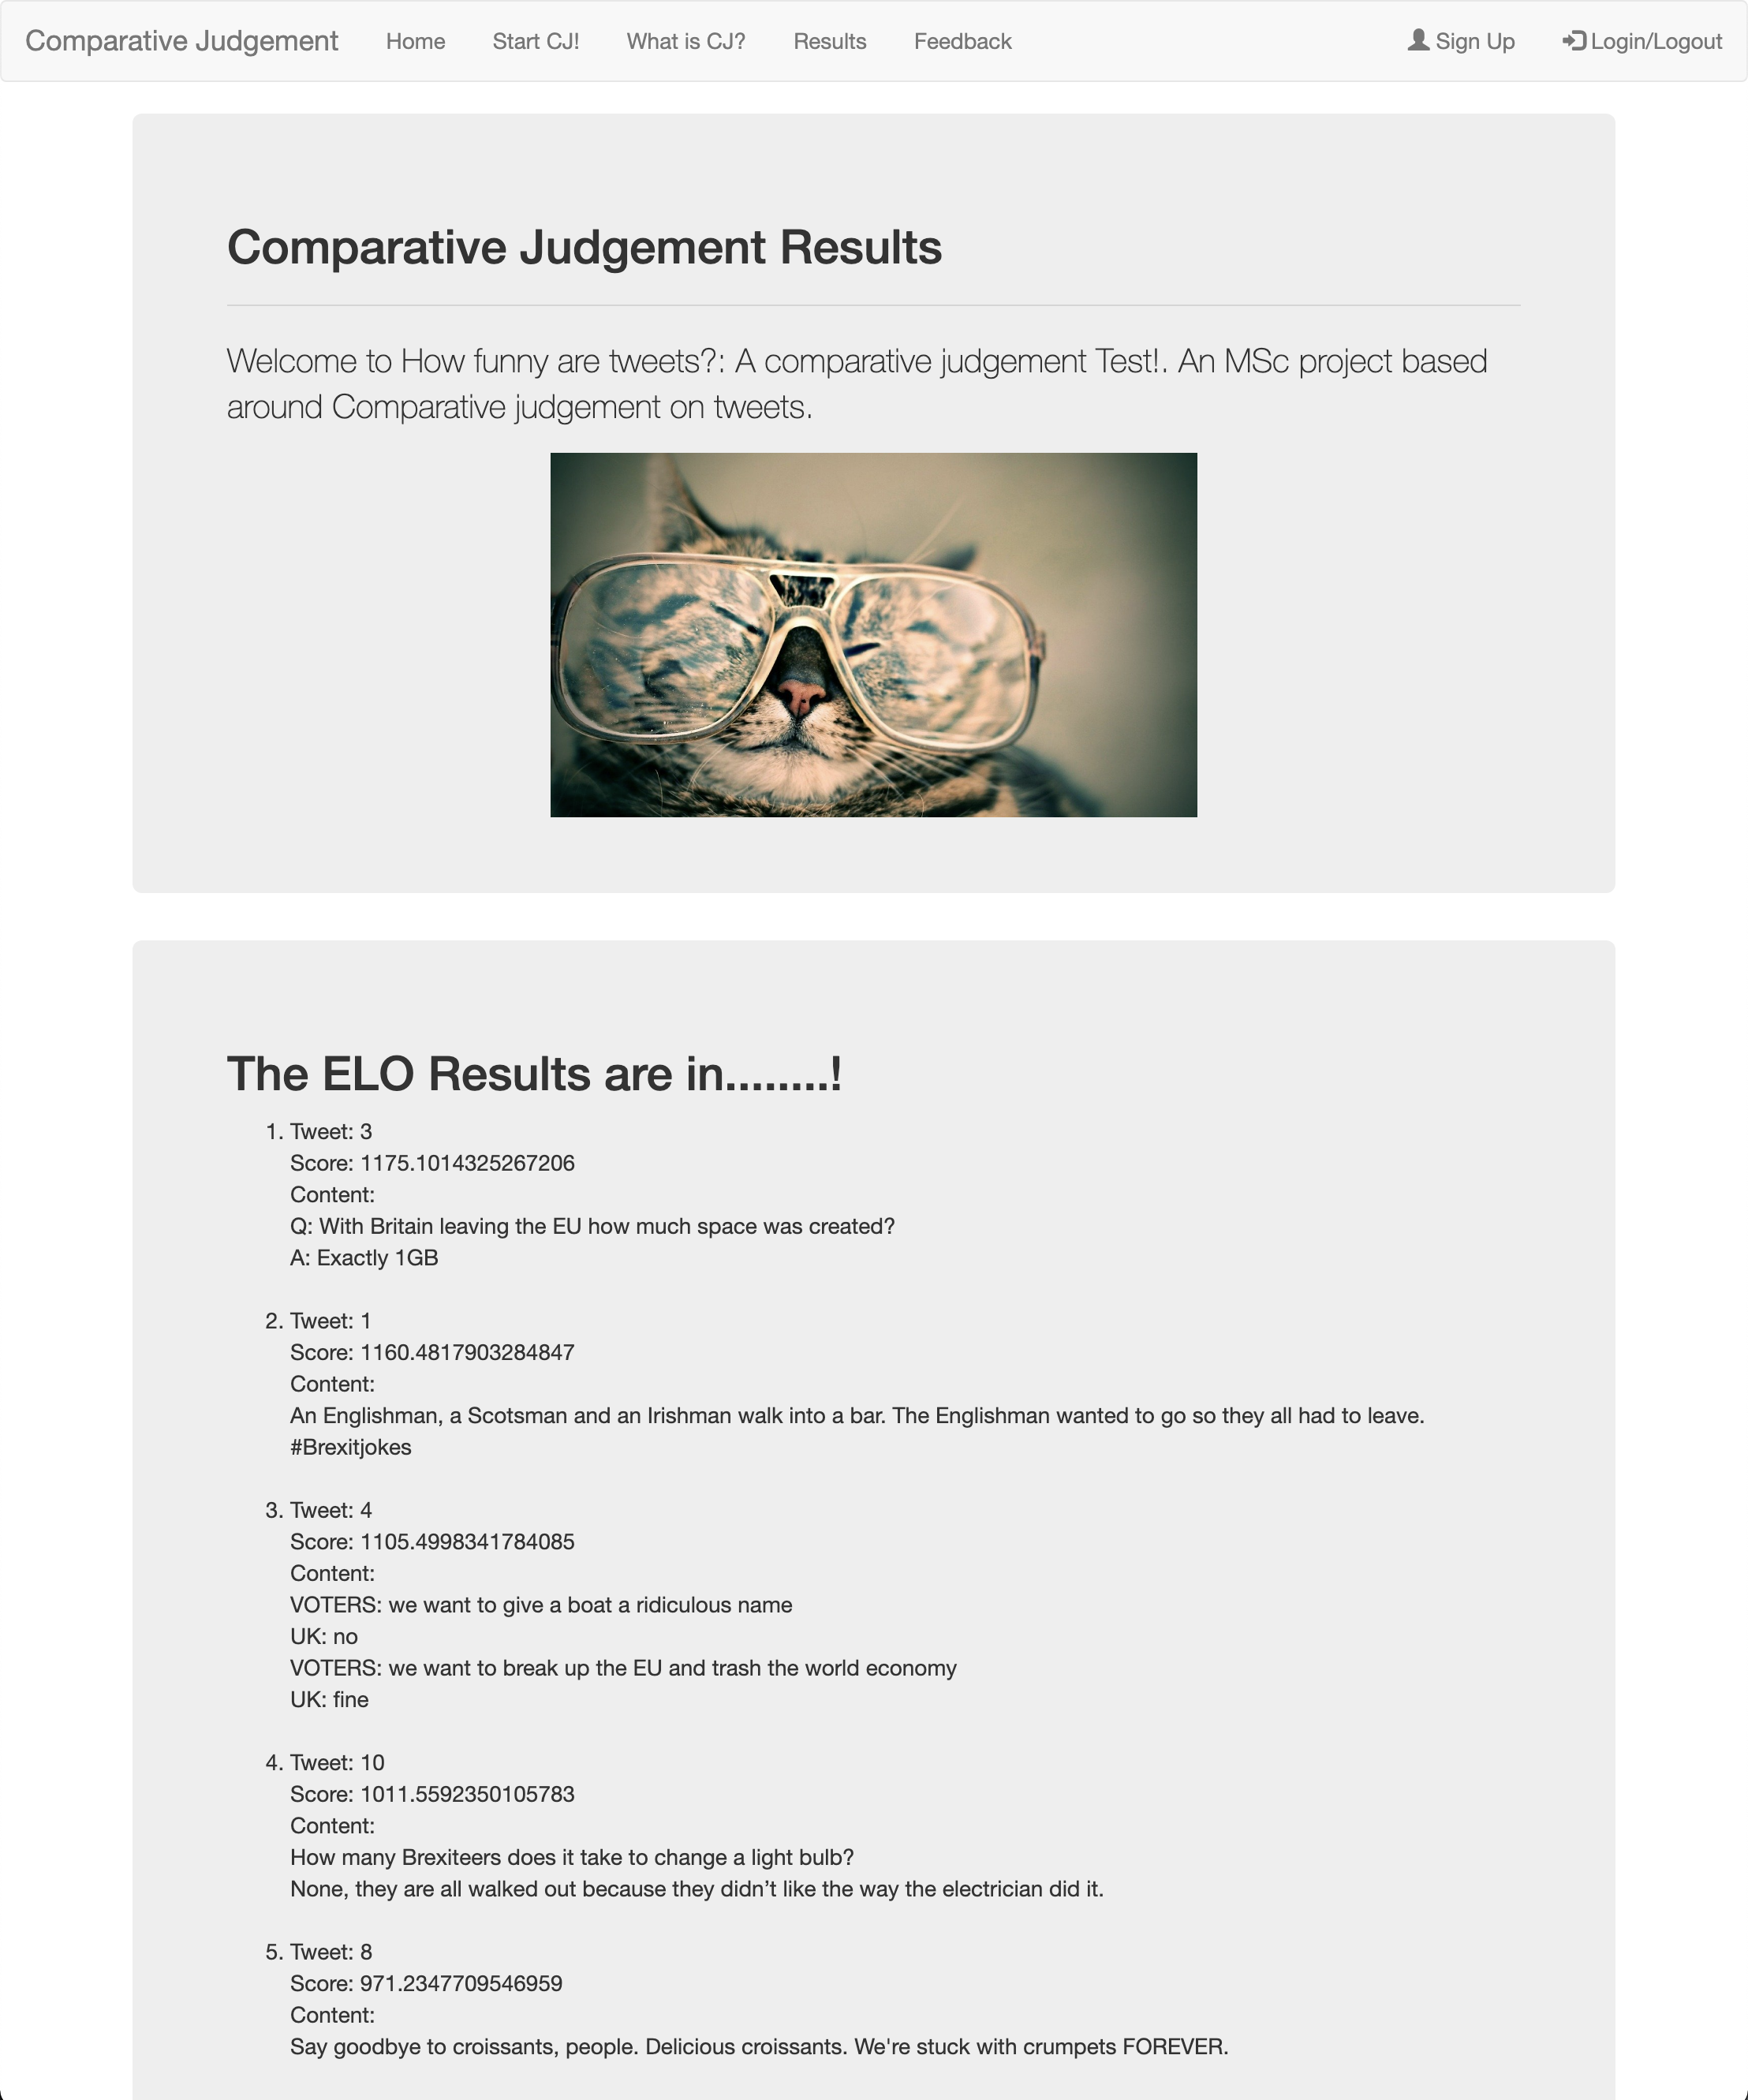
\includegraphics[width=10cm]{Results.png}
	\caption{}
	
		
	\end{figure} 

%\begin{figure}[h]
%	\centering
%	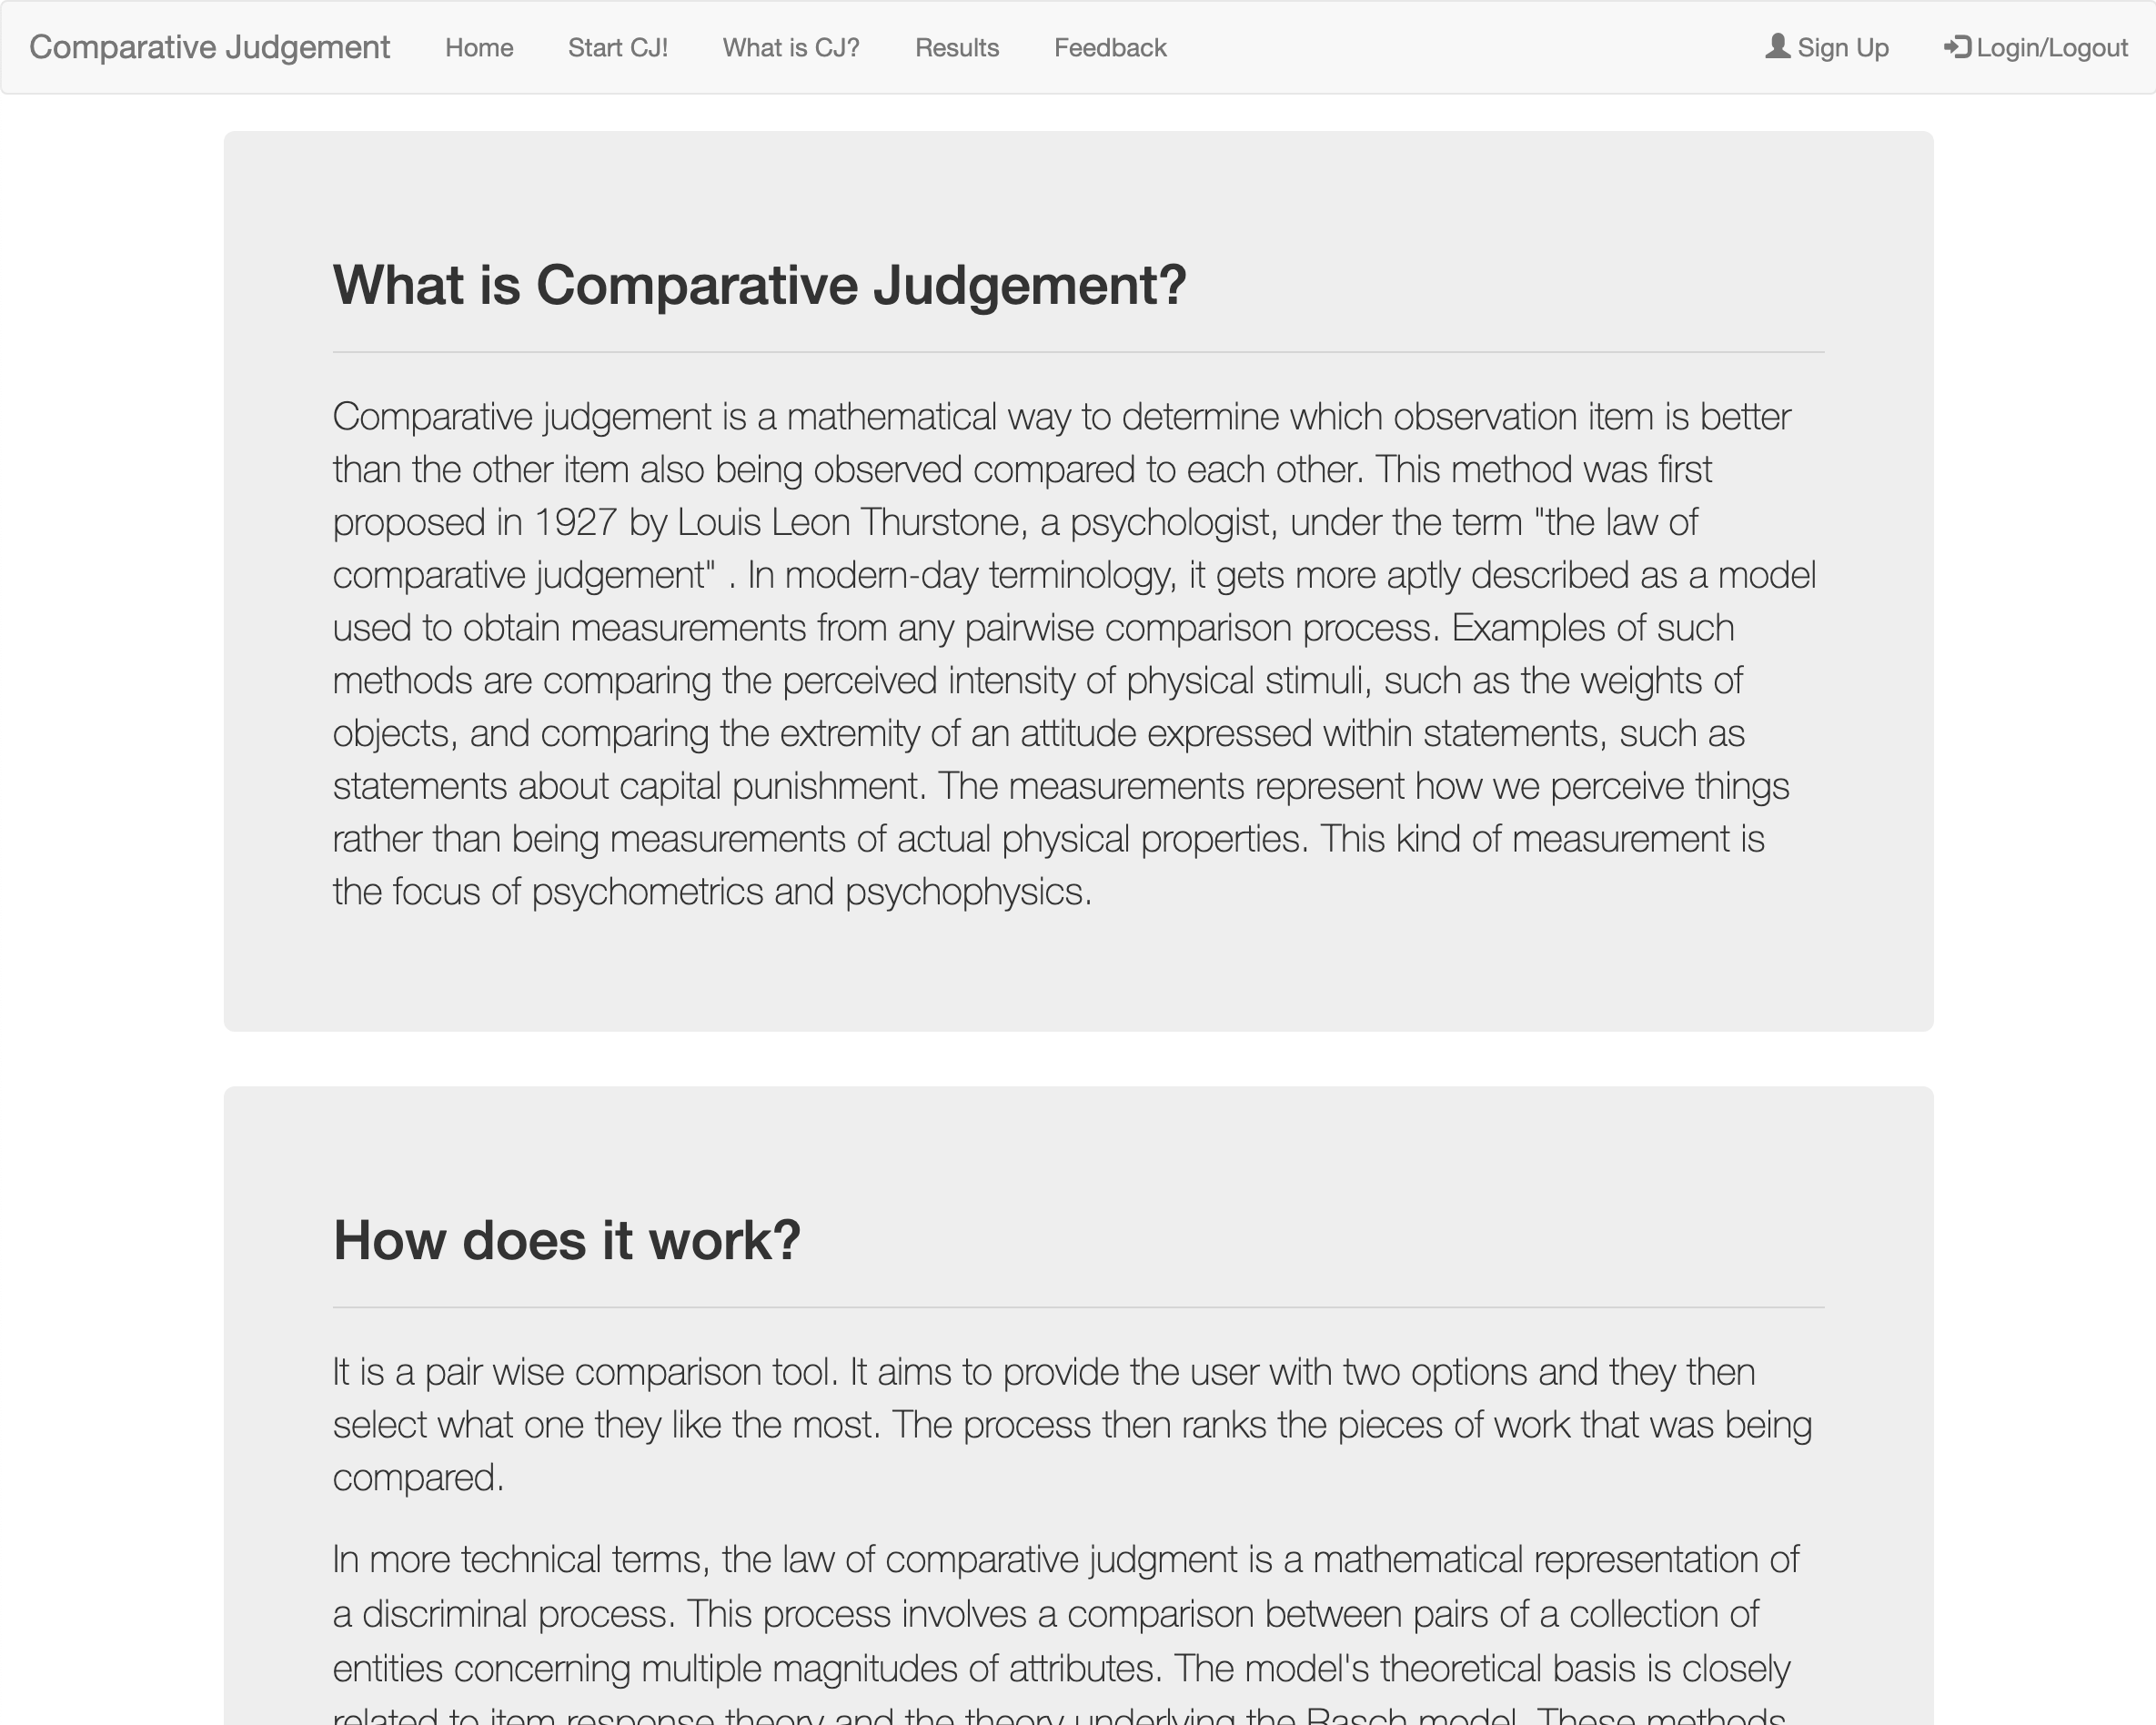
\includegraphics[width=10cm]{What_is_CJ.png.png}
%	\caption{}

		
%	\end{figure} 
\begin{figure}[h]
	\centering
	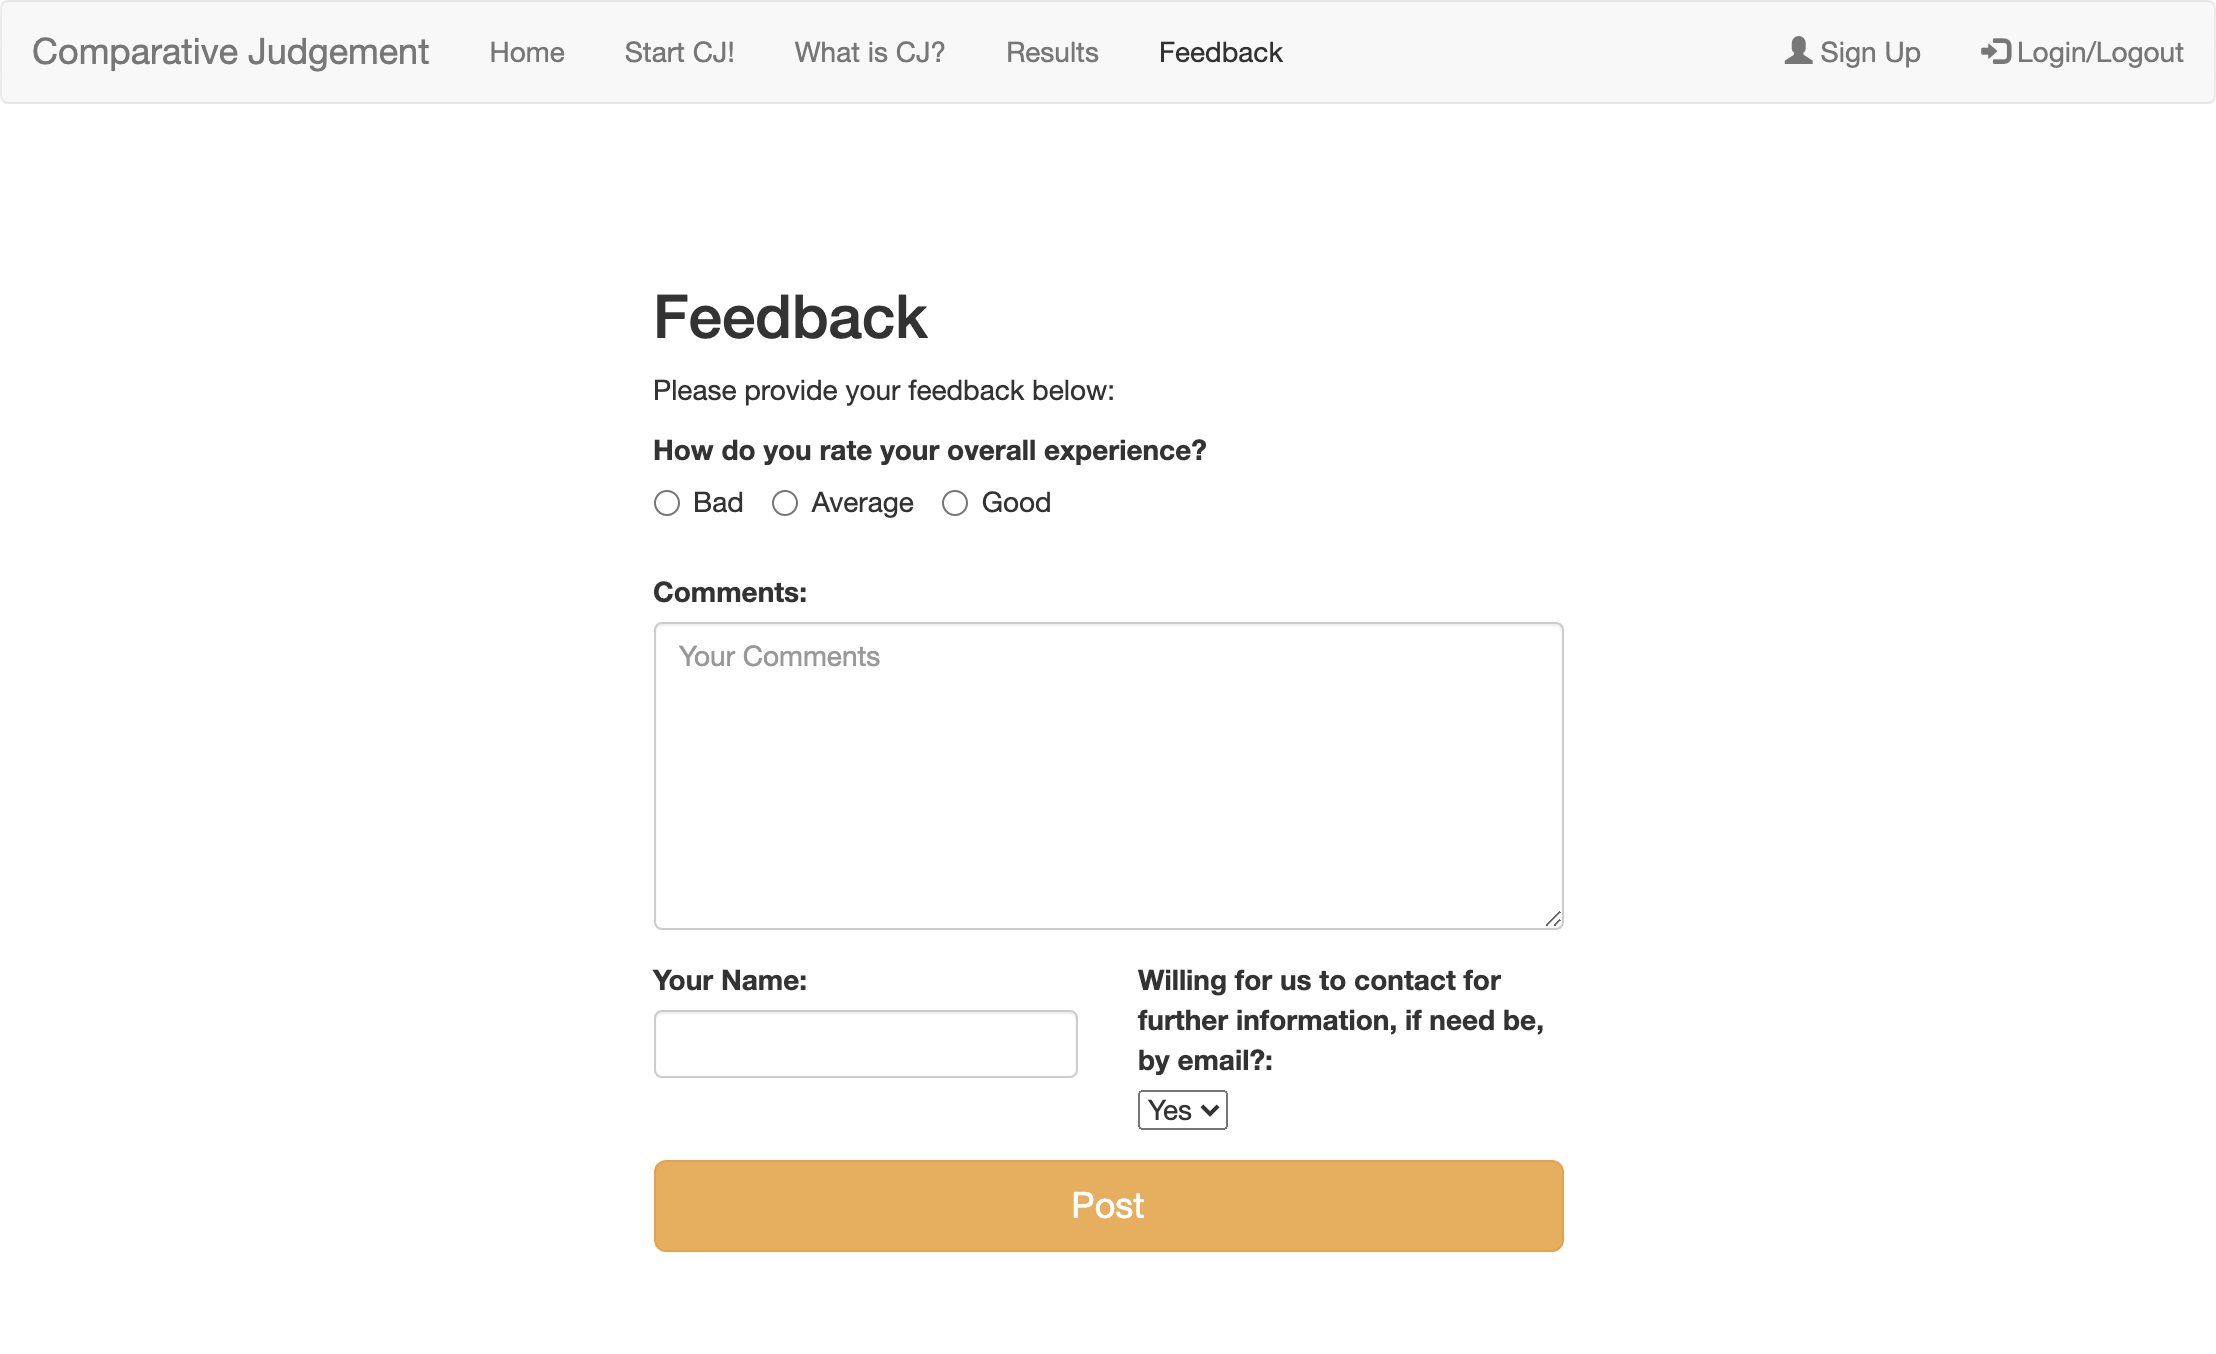
\includegraphics[width=10cm]{feedback.png}
	\caption{}
		
	\end{figure} 

%\begin{figure}[h]
%	\centering
%	\includegraphics[width=10cm]{login.png}
%	\caption{}
	
%\end{figure} 


%\begin{figure}[h]
%	\centering
%	\includegraphics[width=10cm]{signup.png}
%	\caption{}
	
%\end{figure} 

\chapter{Designs}
We will next look at the initial designs compared against the file outcome of the web app. We will also explain the decisions made and what changes we made, and why. 

In total, there are five different pages within the web app. The web app has a home page, facilitates the comparative judgment procedure, results, and feedback.

\subsection{Home Page}

\subsection{Comparison Page}

\subsection{What is Comparative Judgement Page}

\subsection{Results Page}

\subsection{Feedback Page}


\chapter{Risks}


\begin{center}
	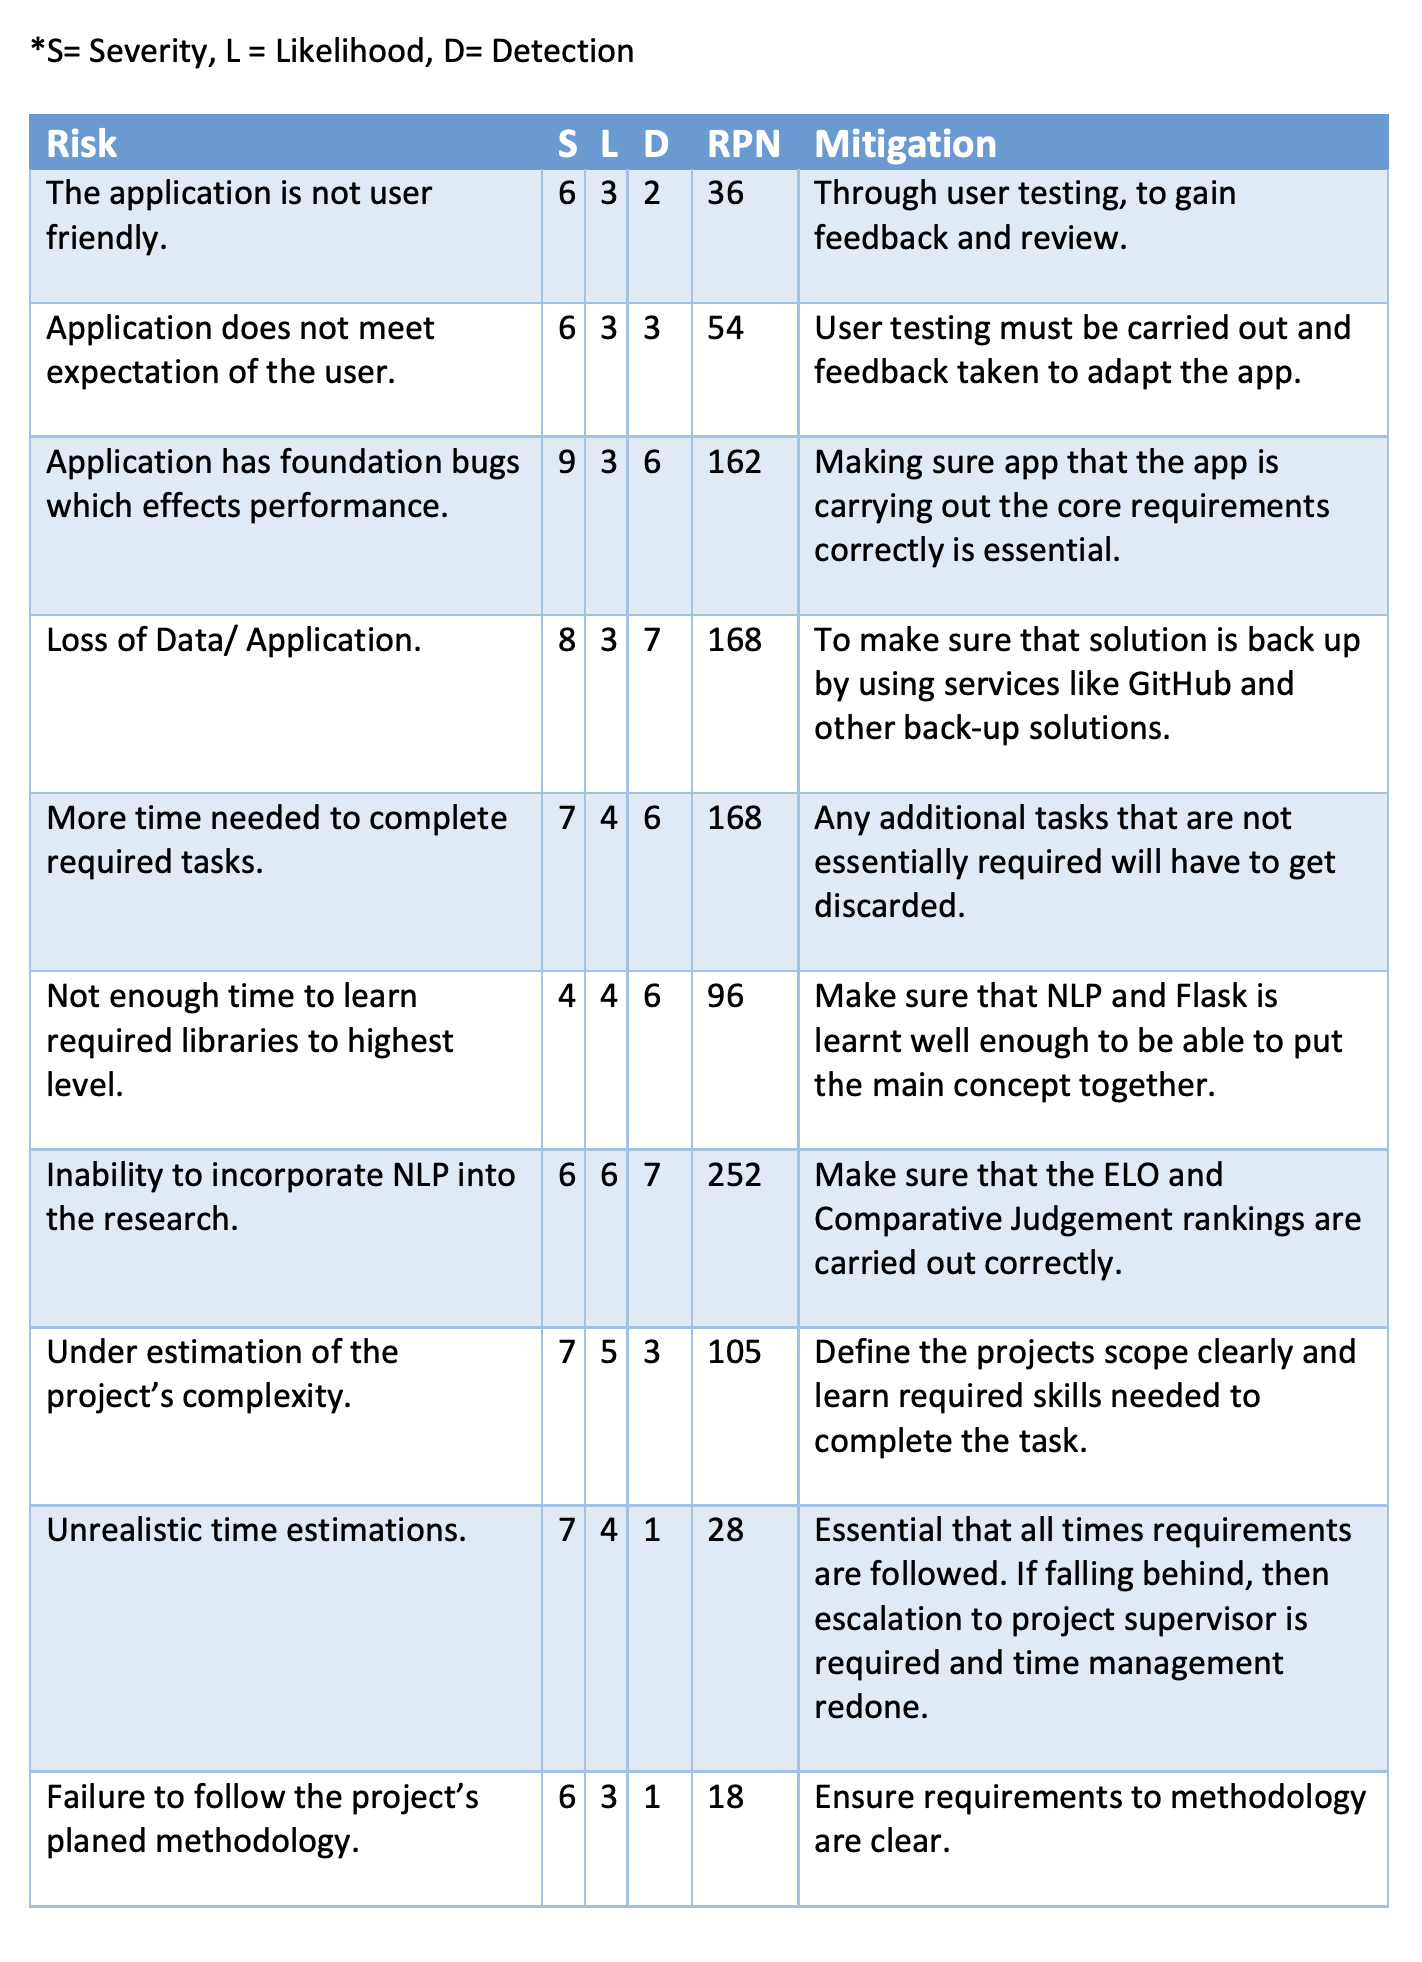
\includegraphics[width=13cm]{risk_table.png}
	%\caption{A visual representation of the processes pipline.}...
\end{center}



\chapter{Schedule}
\begin{landscape}
	
	\begin{center}
		\item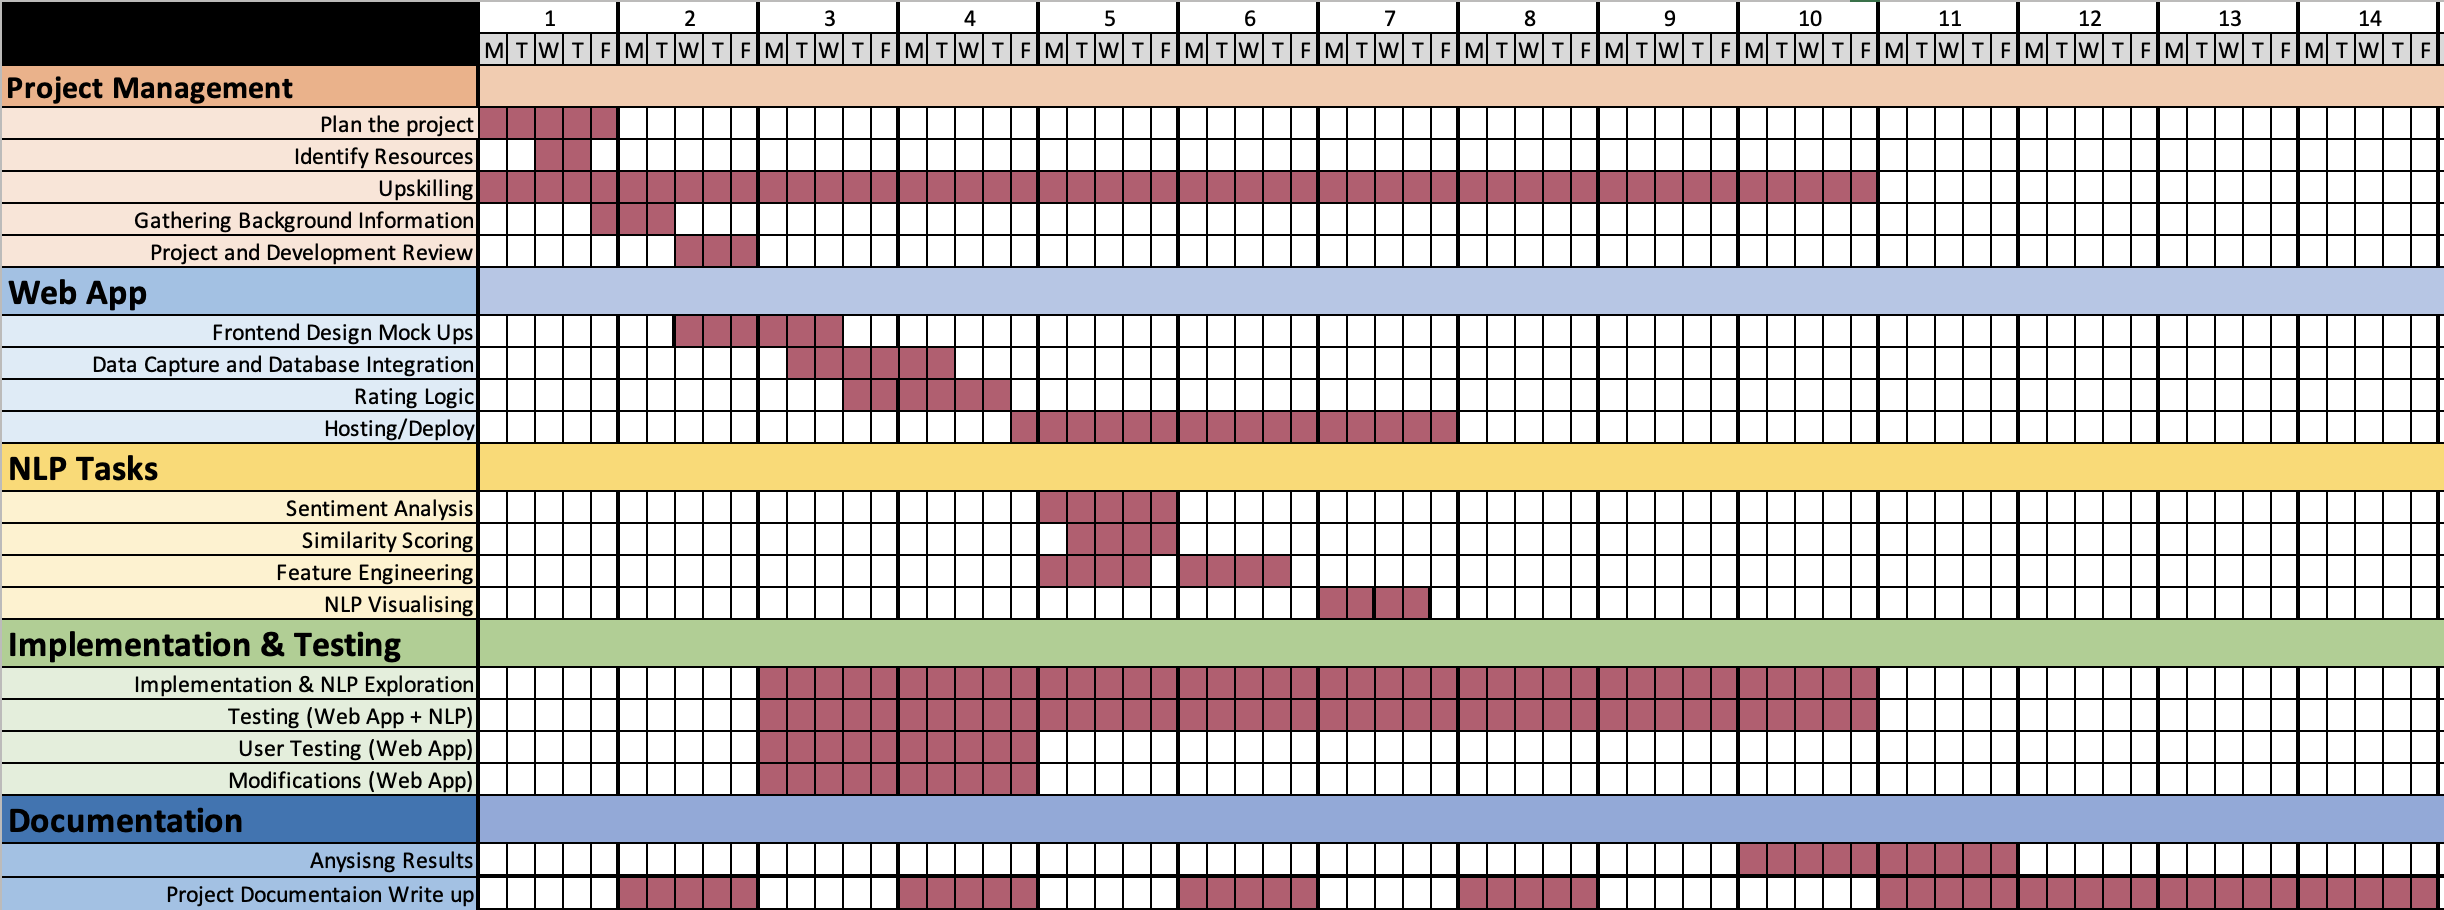
\includegraphics[width=21cm]{ganttchart.png}
	\end{center}
\end{landscape}

\chapter{Software Development Life Cycle Methodology}
Project management is crucial for any task that is about to be carried out, even more so for software development. As a famous Benjamin Franklin quote says, "Failing to plan is planning to fail" \cite{plan_to_fail}. With this in mind, we must decide on the suitable project planning method that compliments our initial software design. From the waterfall method to Rapid application development (RAD) or the more modern methods of agile development, there are many methods that we could choose. We will explain the different methods we could use and what would be best for our solution and intended development method.

The profession of the software developer has existed since the first computers, but the practices and methods for developing software have evolved over timer \cite{SDLC}. The approaches have developed over the years to adapt to the ever-changing landscape of software development. The methods, known as software development life cycles (SDLC), vary in approach but fundamentally share the same goal. The main aims of the SDLC are to break the development up into stages. However, what changes with different SDLC is how these stages get carried out. The different stages are planning, requirements, designing and prototyping, software development, testing, deployment, operations, and maintenance \cite{SDLC}.

The first stage, planning, involves resource allocation, capacity planning, project scheduling, cost estimation, and provisioning \cite{SDLC}. The primary outcome of this stage is to have an overall plan of what we have and what we will need to complete our goal within the constraints like costs and times allowed. The second stage, requirements, is where Subject Matter Experts (SMEs.) guide on what would be needed to carry out the stakeholders' requirements \cite{SDLC}. The third stage, design and prototyping, is where the software architects and developers begin to design the software. The outcome of this stage would be documentation on the intended design patterns and design wireframes of the intended final software. The fourth stage, development, is where the software starts to get made based on the decisions made in design and prototyping, following the chosen methodology. The outcome will be testable, tangible software. The fifth stage, testing, is considered the most crucial stage \cite{SDLC}. It is essential to do all the code quality checking, unit testing, integration testing, performance testing and security testing. The sixth but by no means the final stage is deployment. This stage is when the code is ready to be shipped to the client or uploaded to the required app stores. However, the final stage is operations and maintenance. This stage is about ensuring that the software is getting used as it should and that any bugs that did not initially get picked up in testing are correct and removed from the software. 

%\subsubsection{Waterfall Method}
The waterfall method is a model where each section needs to be completed before moving onto the next stage, like a waterfall flowing down. For example, before we can start analysing the requirements, we need to complete the planning stage. Following the seven critical stages of SDLC, one after the other.

Like all models, they have their advantages and disadvantages. Advantages that this model has is that it is easy to use and follow, and by the way it is all set up, every stage will get finished before the next stage starts. The waterfall method also allows for the project to be easily managed, resulting in easier documentation \cite{cscm01slidesl5}. However, some of the disadvantages are that it is not very useful if the requirements are not very clear at the beginning. Another disadvantage is that once we have moved to the next stage, it is tough to go back to a previous stage to make any changes which therefore creates higher risks to development and has less flexibility \cite{cscm01slidesl5}. The model is best when changes in the project are stable, and the project is small, with the project requirements are clearly defined.

%\subsubsection{RAD: Rapid Application Development}
The overall aim of RAD is to create software projects with higher quality and faster by gathering requirements through workshops or focus groups. Then prototyping the product and then using reiterative user testing of designs early. RAD is the best model for when we need something created quickly and have a pool of users available to test prototypes. However, this approach can be costlym \cite{cscm01slides}. 

%\subsubsection{Spiral Method}
The Spiral Model is an SDLC methodology that aids in choosing the optimal process model. It combines aspects of the incremental build model, waterfall model and prototyping model but is different by a set of six invariant characteristics \cite{spiralmodel}. The Spiral Model main focus is on risk awareness and management. The risk-driven approach of the spiral model ensures the team is highly flexible within its approach and highly aware of the challenges they can expect down the road. The spiral model shines when stakes are highest, and significant setbacks are not an option \cite{spiralmodel}.


%\subsubsection{Agile Development}
The Agile methodology is a process by which a team can manage a project, which gets achieved by breaking up the project into several stages. It required constant collaboration with stakeholders, which leads to continuous iterations of improvement. In essence, Agile development is not a set methodology more of a manifesto aiming to uncover better ways to develop software. "Individuals and interactions over processes and tools. Working software over comprehensive documentation. Customer collaboration over contract negotiation. Responding to change over following a plan \cite{agilemanifesto}."

%\subsubsection{Decided Method}
The project's requirements have features that lend themselves well to the waterfall methodology. However, we would like to have an element of agile methodology within the development due to the application intending to get created in a modular way. Using the waterfall method will allow us to have a clear plan and requirements of what is needed, but by using the agile method, we can rotate between the software development and testing stages.

\chapter{Testing}

The web application was the part of the implementation that required rigorous testing. The testing was because the web app was the bit that users would be interacting with the study. Therefore, we needed to ensure the app was to a high standard not to detract away from the users' experience and solely focus on the application purpose, which is to select which tweet they think is funnier. 

We conducted multiple in-house testing using an internal server's localhost to ensure that the app was suitable. Additionally, we allowed a small number of users to test out the application. Once we were happy with the feedback, the application's data got reset and published to potential users.

